\section{Results}
\label{sec:results}

The data-driven probabilistic model we have presented can be applied in many different ways to produce diverse coloring suggestions. The factor graph representation makes it easy to adapt our framework to handle new problems or incorporate user-provided design constraints by introducing additional factors to the factor graph, or changing the source data used to train the factor weights and histograms.

\remark{Discuss parameters used to train model ``unless otherwise specified''. Number of artists, weights, etc. Say that the supplemental materials lists the patterns used in this training set.}
\remark{Because many patterns are recolorings of the same template, we make sure to separate our training and test sets so they do not share any templates}

The results shown below are rendered using the color assignments generated by our model, with the COLOURlovers interface. 
%The results shown below are rendered from the original vector pattern using the Colourlovers interface, from color assignments generated by our model. 

\subsection{Coloring Pattern Templates}

\paragraph{Automatic pattern coloring} In the most direct application of our framework, we can sample from our model to produce colorings for a pattern template that are similar to the colorings used for training. Figure~\ref{fig:teaser} shows two examples of this process. The sampled patterns exhibit a range of colors and styles employed by the Colourlover artists. For comparison, the same patterns colored with palettes randomly sampled from RGB-space are shown on the right. These patterns exhibit significant problems, such as low color harmony and adjacent regions with equi-limuinant colors.

\begin{figure*}[ht]
\begin{tabular}{ccc}

\includegraphics[width=.15\linewidth]{figs/permutationTemplatePalette} & 
\includegraphics[width=.4\linewidth]{figs/permutationBest8} & 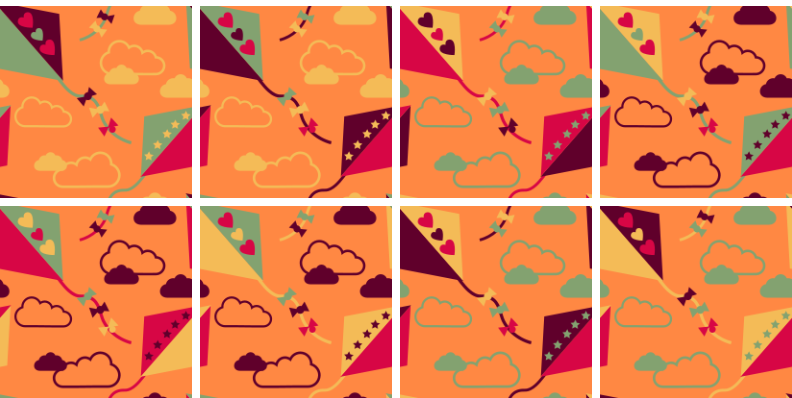
\includegraphics[width=.4\linewidth]{figs/permutationWorst8} %& 
\includegraphics[width=.12\linewidth]{figs/permutationArtist}
  \\
\textbf{(a)} Input Pattern & \textbf{(b)} Highest-scoring assignments & \textbf{(c)} Lowest-scoring assignments %& \textbf{(d)} Artist assignment
\\
\end{tabular}

\caption{Given a segmented image and corresponding palette as input, we use our color model to compute the likelihood of each possible assignment of the palette to the image regions. \textbf{(b)} and \textbf{(c)} show the top-eight and bottom-eight assignments. The assignment provided by the artist received the second-highest score and is highlighted in blue.}
\label{fig:permutation}
\end{figure*}


\begin{figure}[ht]
\begin{tabular}{cccc} 
\raisebox{0.5em}{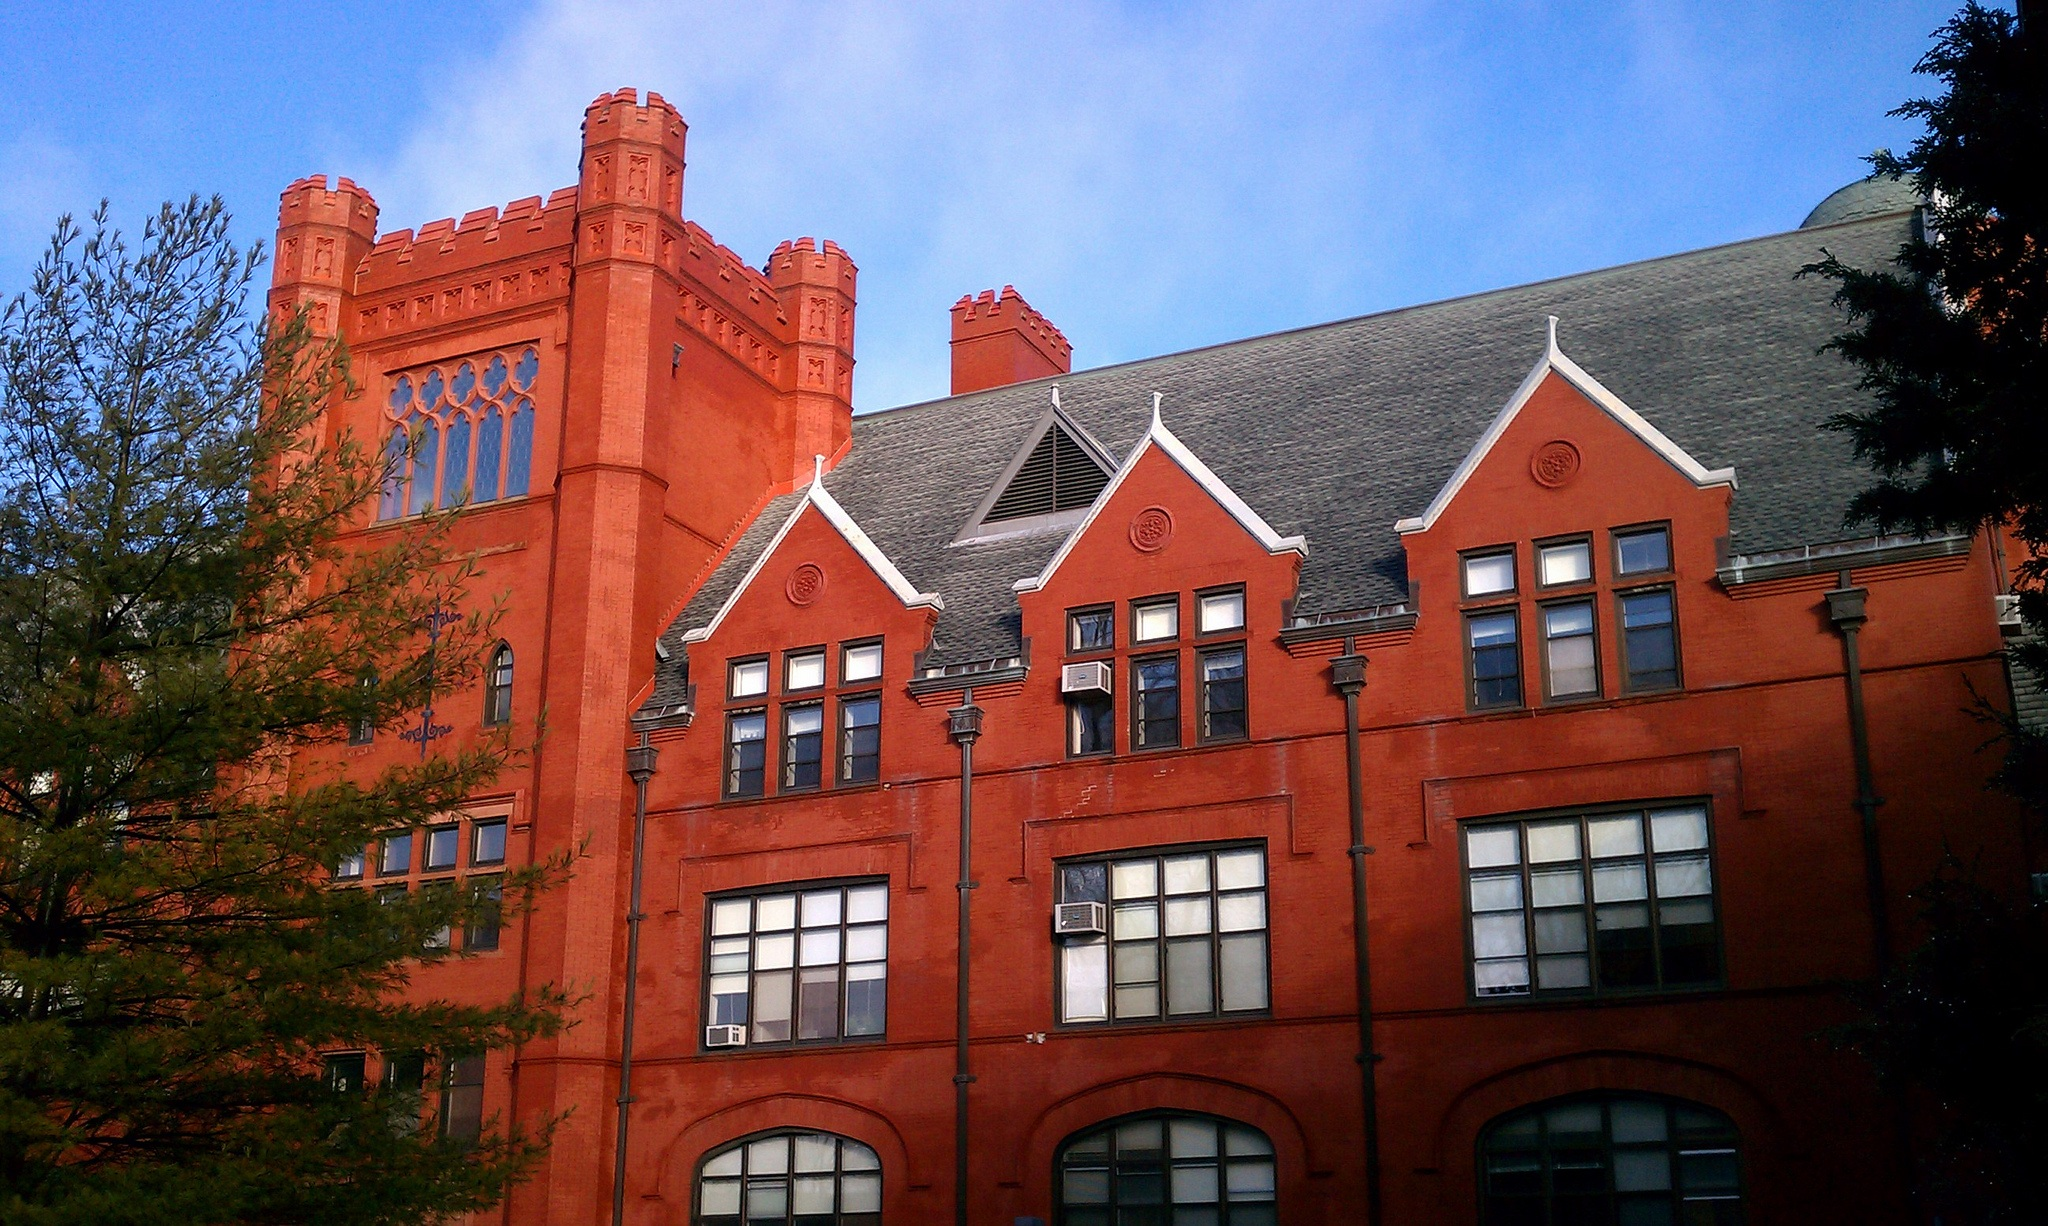
\includegraphics[width=.275\columnwidth]{figs/photos/brick}}&
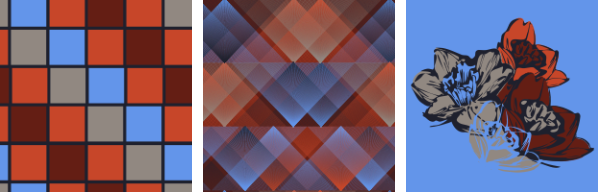
\includegraphics[width=.65\columnwidth]{figs/photos/brickAll}\\
\raisebox{0.5em}{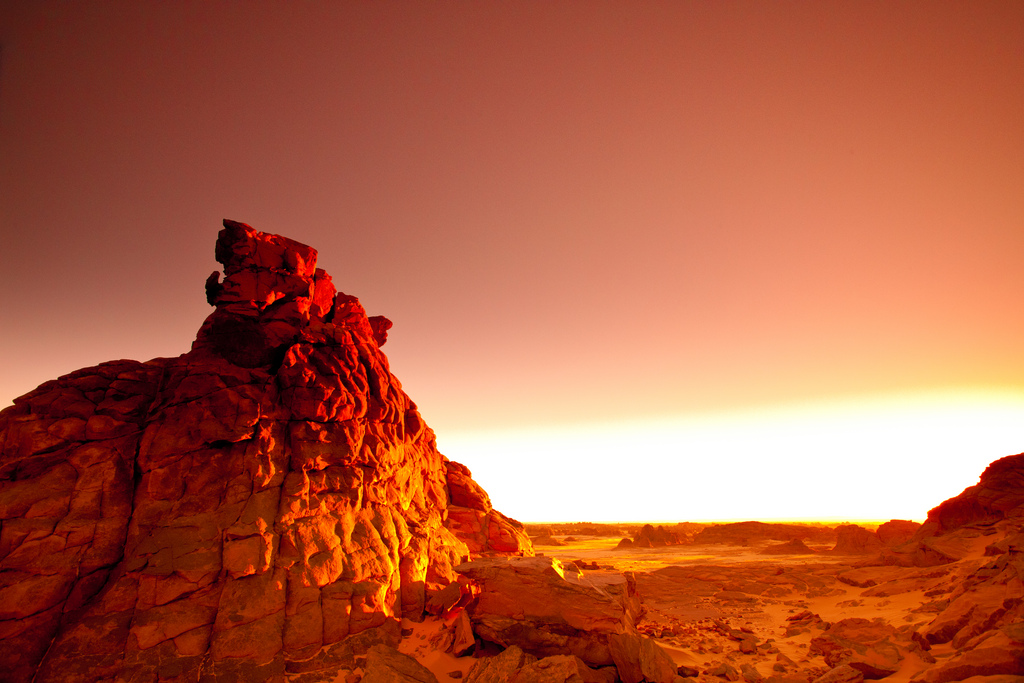
\includegraphics[width=.275\columnwidth]{figs/photos/sunset}}&
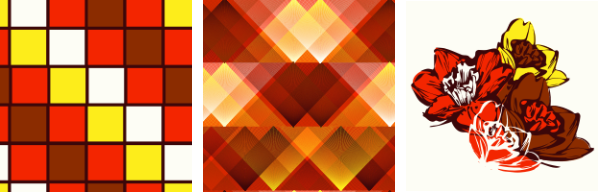
\includegraphics[width=.65\columnwidth]{figs/photos/sunsetAll}
\end{tabular}

\caption{Palettes are extracted from the two input photographs on the left, and on the right we show the top-scoring coloring suggested by our algorithm for three different pattern templates.}
\vspace{-1.0em}
\label{fig:photographMatching}
\end{figure}

\paragraph{Coloring with fixed palettes} In some cases, an artist already knows what colors she wants to use in an image. She might have found an appealing palette elsewhere or may have a very specific theme in mind. Even with a fixed palette, there are still a range of images that can be created by mapping different colors to different regions, only some of which are desirable. To support this task, we use our model's score to rank all possible permutations of the colors. Figure~\ref{fig:permutation} shows one example of this process. \ref{fig:permutation}b shows the eight highest-rated color assignments which exhibit a variety of color styles, such as using four different background colors. On the other hand, the lowest-rated assignments all use the tangerine background color. Our color model assigns a very low score to using this color for the background region because its color properties are not similar to background colors in the training set. The actual color assignment originally provided by the artist for this color template received the second-highest score, suggesting that our model was able to capture the artist's intent. Figure~\ref{fig:photographMatching} shows another application, where the input palette is instead derived from an input photograph~\cite{SharonPaletteExtraction}. Our algorithm automatically computes a pleasing mapping from the colors in the extracted palette to regions in a given pattern template.

\paragraph{Hard color constraints}

\begin{figure*}[ht]
\begin{tabular}{cc} 
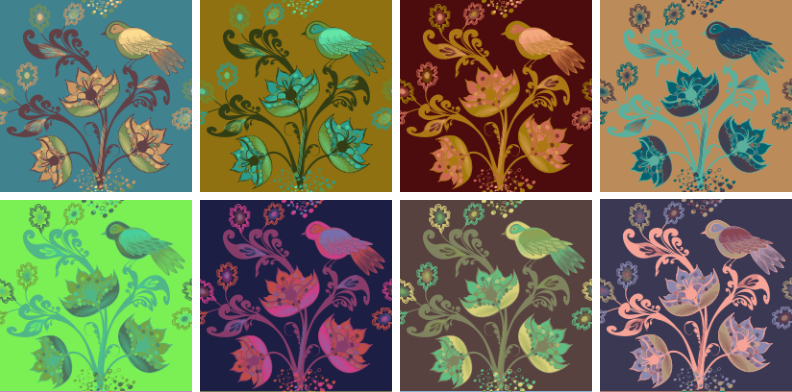
\includegraphics[width=.475\linewidth]{figs/constrainedSearchUnconstrained}&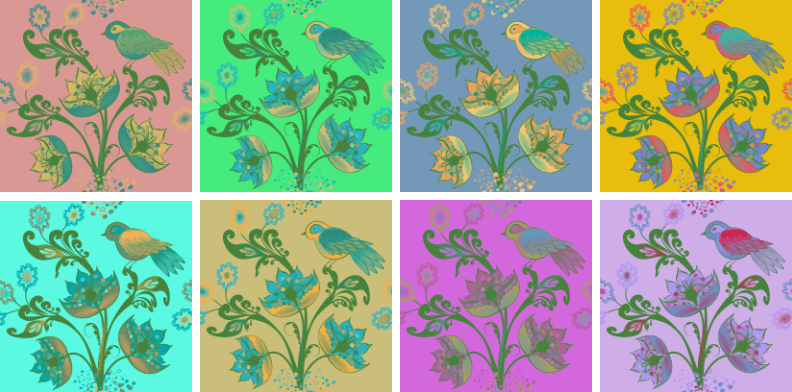
\includegraphics[width=.475\linewidth]{figs/constrainedSearchConstrained}\\
Unconstrained sampling&Constrained sampling\\
\end{tabular}

\caption{An artist coloring a pattern is presented with the results shown on the left, and decides that she only likes results where the stem of the plant is dark green. On the right, we use conditional inference to sample from our model subject to the constraint that the desired palette entry is fixed to a specific color. This is a natural way to incorporate semantic information about region colors which our model cannot capture.}
\label{fig:constrainedInference}
\vspace{-1.0em}
\end{figure*}

A user coloring a pattern may be confident about the colors he wants to see in some regions but uncertain about others. Our model can assist users in this situation by fixing the color of certain pattern regions and using conditional inference to sample values for the remaining unconstrained color variables. Figure~\ref{fig:constrainedInference} shows an example, in which the model samples from the highest-scoring patterns subject to the constraint that the plant stem must be a specific shade of green.

\paragraph{Soft color constraints}

In another use case, a user might manually color a pattern and then wish to see variations upon this theme, hoping to find better-looking alternatives nearby in the space of colorings. Our model can support this type of query by incorporating an additional soft constraint factor on color variable, constraining it ot be close to a target color:
%%
\begin{equation}
\factor^\textrm{Target}(\colorVars_\group | \pattern) = \mathcal{N}(||\colorVars_\group - \textrm{targetColor}(\group)||, \sigma_\textrm{user})
\label{eq:targetFactor}
\end{equation}
%%
Here, $\textrm{targetColor}(\group)$ is the desired color of group $\group$ and $\sigma_\textrm{user}$ controls the extent to which the group is allowed to deviate from the desired color. We assign this factor a weight $w_\textrm{user} * w_\textrm{model}$, where $w_\textrm{model}$ is the sum of the weights of all other factors in the model. $w_\textrm{user}$ controls the tradeoff between satisfying the user-specified target colors for a region versus satisfying the color distribution encoded by the trained model.
%
%This factor corresponds to adding a new term in our log-linear model with this statistics function:
%%%
%\begin{equation*}
%\termStats(\colors | \pattern) = \sum_{\group \in \groups}{\ln \mathcal{N}(||\colors_\group - \textrm{targetColor}(\group)||, \sigma_\textrm{user})}
%\end{equation*}
%%%

\begin{figure}[ht]
\begin{tabular}{cc}
{
\includegraphics[width=.1785\columnwidth]{figs/guidedSearch1Original}}&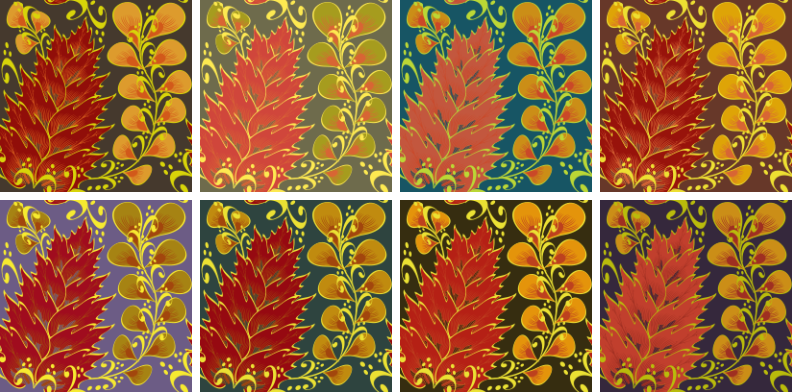
\includegraphics[width=.735\columnwidth]{figs/guidedSearch1MMR}\vspace{0.5em}\\
{
\includegraphics[width=.1785\columnwidth]{figs/guidedSearch0Original}}&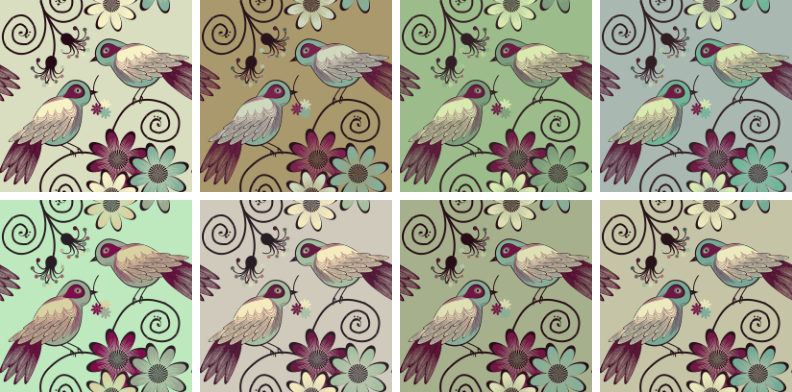
\includegraphics[width=.735\columnwidth]{figs/guidedSearch0MMR}\vspace{0.5em}\\
%\raisebox{2em}{
\includegraphics[width=.22\columnwidth]{figs/guidedSearch2Original}}%&
\includegraphics[width=.7\columnwidth]{figs/guidedSearch2MMR}\\
Original&Suggestions\\
\end{tabular}

\caption{An artist provides an initial color assignment and asks for patterns that are similar. We incorporate this request by adding an additional factor to our model, showing four samples drawn from the new model for each of the input images.}
\label{fig:nearbySuggestions}
\vspace{-1.0em}
\end{figure}

Figure~\ref{fig:nearbySuggestions} shows example scenarios where a proposed coloring is given, and the model returns similar colorings. Our model is able to make significant variations to the input colors while still preserving desirable properties of the results.

\begin{figure}[ht]
\begin{tabular}{ccc} 
Style&Example&Results\\ %\hline
\raisebox{1.55em}{\emph{Light}}&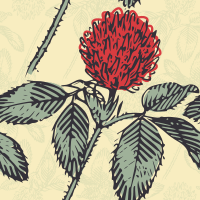
\includegraphics[width=.148\columnwidth]{figs/styleResultsLightExample}&
\includegraphics[width=.62\columnwidth]{figs/styleResultsLight}\vspace{0.5em}\\
\raisebox{1.55em}{\emph{Dark}}&
\includegraphics[width=.148\columnwidth]{figs/styleResultsDarkExample}&
\includegraphics[width=.62\columnwidth]{figs/styleResultsDark}\vspace{0.5em}\\
\raisebox{1.55em}{\emph{Bold}}&
\includegraphics[width=.148\columnwidth]{figs/styleResultsBoldExample}&
\includegraphics[width=.62\columnwidth]{figs/styleResultsBold}\vspace{0.5em}\\
\raisebox{1.55em}{\emph{Mellow}}&
\includegraphics[width=.148\columnwidth]{figs/styleResultsMellowExample}&
\includegraphics[width=.62\columnwidth]{figs/styleResultsMellow}\vspace{0.5em}\\
\end{tabular}

\caption{In this example, 17 patterns were chosen in three different styles, and a representative image from each style is shown in the second column. A separate model was then trained on each style, and in the third column we show four samples drawn from each model. In each case, our model is able to learn different properties of the desired distribution over colors.}
\label{fig:styleTraining}
\vspace{-1.0em}
\end{figure}

\begin{figure*}[ht]
\begin{tabular}{cc} 
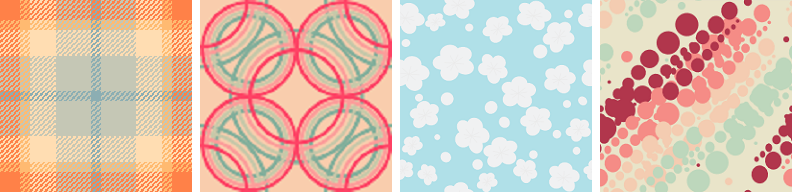
\includegraphics[width=.48\linewidth]{figs/styleSugarExamples}&
\includegraphics[width=.48\linewidth]{figs/styleAlbenajExamples}\vspace{1.0em}\\
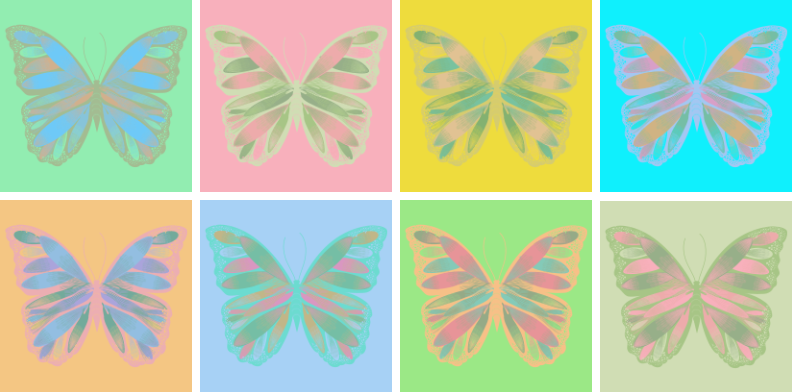
\includegraphics[width=.48\linewidth]{figs/styleSugar}&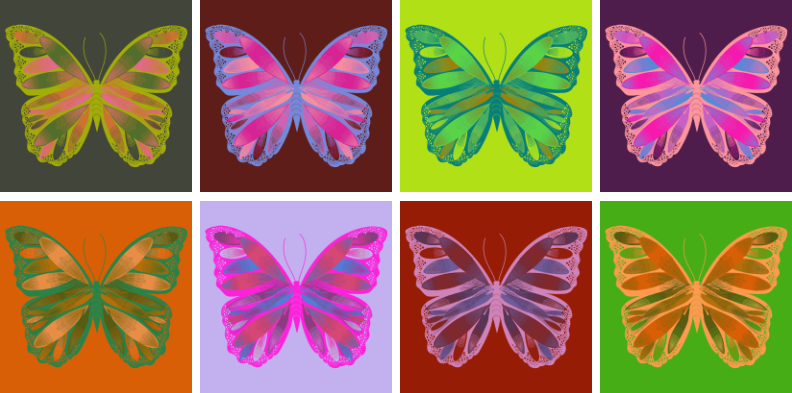
\includegraphics[width=.48\linewidth]{figs/styleAlbenaj}\\
Artist A&Artist B\\
\end{tabular}

\caption{Our data-driven approach makes it easy to capture the styles of different artists. Top: representative images from two different artists. Bottom: results sampled from a model trained on 100 images from the artist.}
\vspace{-1.0em}
\label{fig:artistTraining}
\end{figure*}

\paragraph{Style capture} A powerful advantage of a data-driven approach is the ability to modify the underlying training source to achieve specialization of the resulting model. This ability allows our model to capture a specific style and color preferences such as ``high-contrast patterns'' simply by selecting a set of patterns with the desired property. Figure~\ref{fig:styleTraining} demonstrates this behavior using four style categories: \emph{Light}, \emph{Dark}, \emph{Bold}, and \emph{Mellow}. With only 17 training examples, our model can still capture general properties of the example patterns such as the distribution of colors over the background regions in \emph{Light} and \emph{Dark} and the amount of contrast between regions in \emph{Bold} and \emph{Mellow}. The model can also capture the style of a specific artist, as shown in Figure~\ref{fig:artistTraining}. Here, 100 images from each artist were used for training. The sampled images mimic certain properties of the the style of each artist, such as the light backgrounds preferred by artist A and the bold colors and dark backgrounds preferred by artist B. The complete list of patterns used as training data for these examples can be found in the supplemental materials.

\subsection{Applications}

\paragraph{Web design}
A web designer may want to change a web page's color theme to fit the season, a special event, or even the time of day. Our model can support these tasks by suggesting recolorings for web page pattern elements. In Figure~\ref{fig:webpageRecoloring}, the background pattern of a blog is automatically recolored in three distinct styles. Each style is defined by a manually-specified page body color and header text color. We generate these recolorings by adding new factors to the model. First, we add a unary factor to each color variable that encourages it to be similar to a color that occurs in the web page body:
%%
\begin{equation*}
\factor^\textrm{WebSim}(\colorVars_\group | \webpage) = p(\colorVars_\group | \webpage)
\end{equation*}
%%
where $\webpage$ is a rendered image of the web page body. The distribution $p$ is represented with a smoothed histogram of colors in the image, after quantizing to a small number of colors (20, in this experiment).
We also add a factor to the pattern's background color group (assumed to be the largest color group in the pattern) that penalizes it for being too similar to the web page body background color:
%%
\begin{equation*}
\factor^\textrm{BgPen}(\colorVars_{\textrm{largest}(\groups)} | \webpage) = 0.05 \cdot || \colorVars_{\textrm{largest}(\groups)} - \textrm{bgColor}(\webpage) ||
\end{equation*}
%%
Incoporating this term ensures that the body of the page stands out from the rest of the page. A more sophisticated approach would consider the entire web page to be a pattern and perform joint recoloring; we leave this extension to future work.


\begin{figure}[ht]
\centering

\includegraphics[width=\columnwidth]{figs/webpageRecoloring}
\caption{With a few additional factors, our model can recolor the background pattern of a web page to match the colors in the page body.}
\label{fig:webpageRecoloring}
\end{figure}

\paragraph{3D scene design}
Color-coordinating a virtual scene is another creative task that can benefit from computatational support. While repositories such as the 3D Warehouse provide a wealth of object models with which to build scenes, and prior research has investigated computational support for arranging those objects~\cite{SceneSynth}, coloring them in a consistent and pleasing way remains challenging. Figure~\ref{fig:sceneRecoloring} shows how our model can make this task easier. In this example, the original scene is composed of models whose material colors are internally consistent but do not harmonize with each other; this is a common problem when constructing scenes from repository models. We can treat this scene as a recolorable pattern by rendering its material coefficients to an image. The user then provides a few additional annotations to specify which object components should take the same color; in this example, all cushions, pillows, and wooden objects must take the same color. Finally, we add a factor to our model to enforce that the colors assigned to each component are similar to their original colors (see Equation~\ref{eq:targetFactor}). The resulting model, when sampled, suggests plausible, improved recolorings of the scene. Our model's applicability to this task, despite it being trained only on \emph{2D} patterns, suggests that it captures some simple cross-domain aesthetic principles.

\begin{figure*}[ht]
\begin{tabular}{c|ccc} 
Original&Recoloring 1&Recoloring 2&Recoloring 3\vspace{0.4em}\\
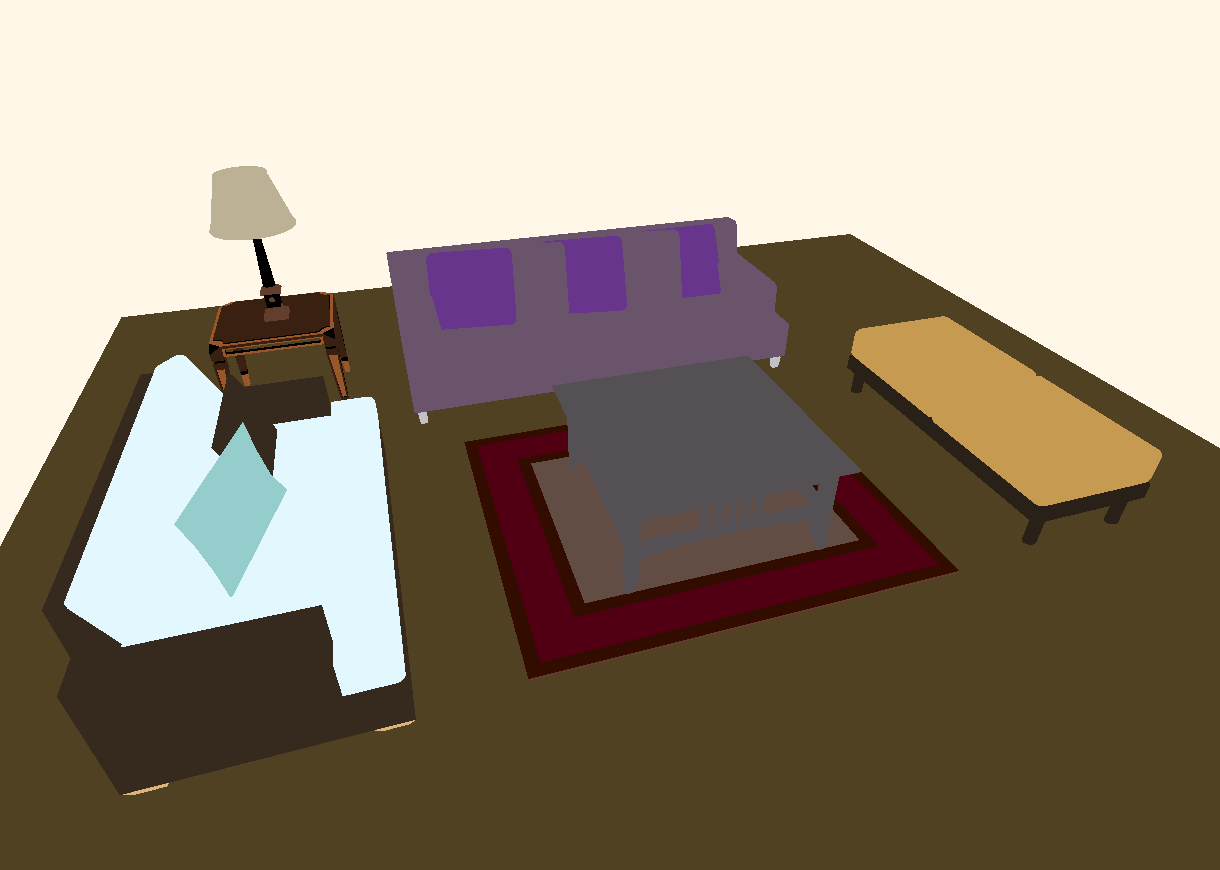
\includegraphics[width=.23\linewidth]{figs/3dscene/original}&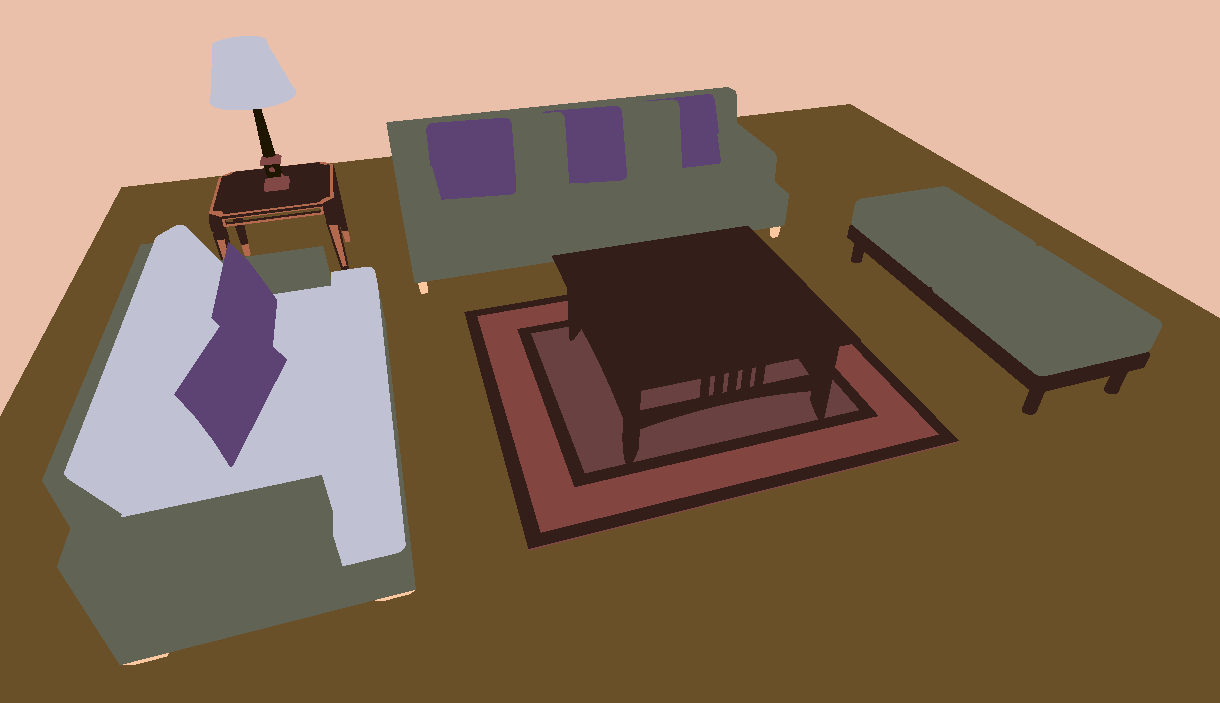
\includegraphics[width=.23\linewidth]{figs/3dscene/recolored_17}&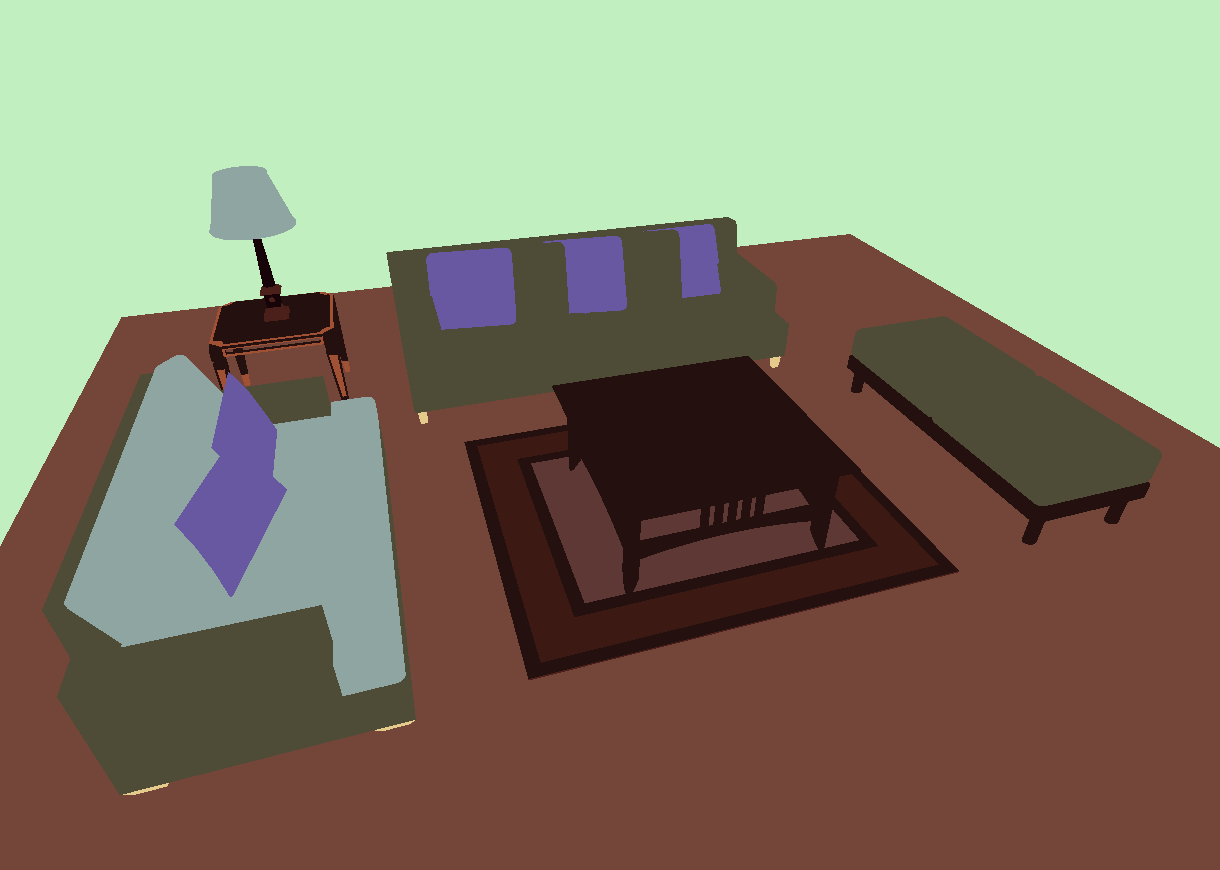
\includegraphics[width=.23\linewidth]{figs/3dscene/recolored_03}&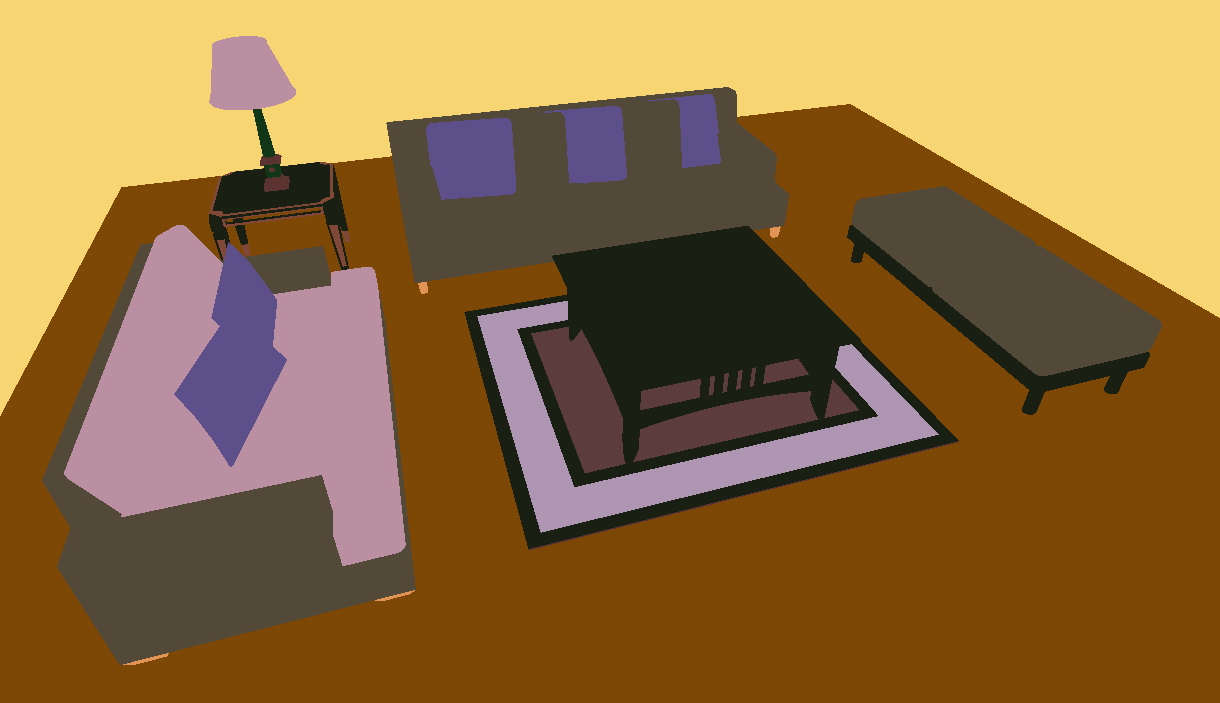
\includegraphics[width=.23\linewidth]{figs/3dscene/recolored_15}\vspace{0.4em}\\
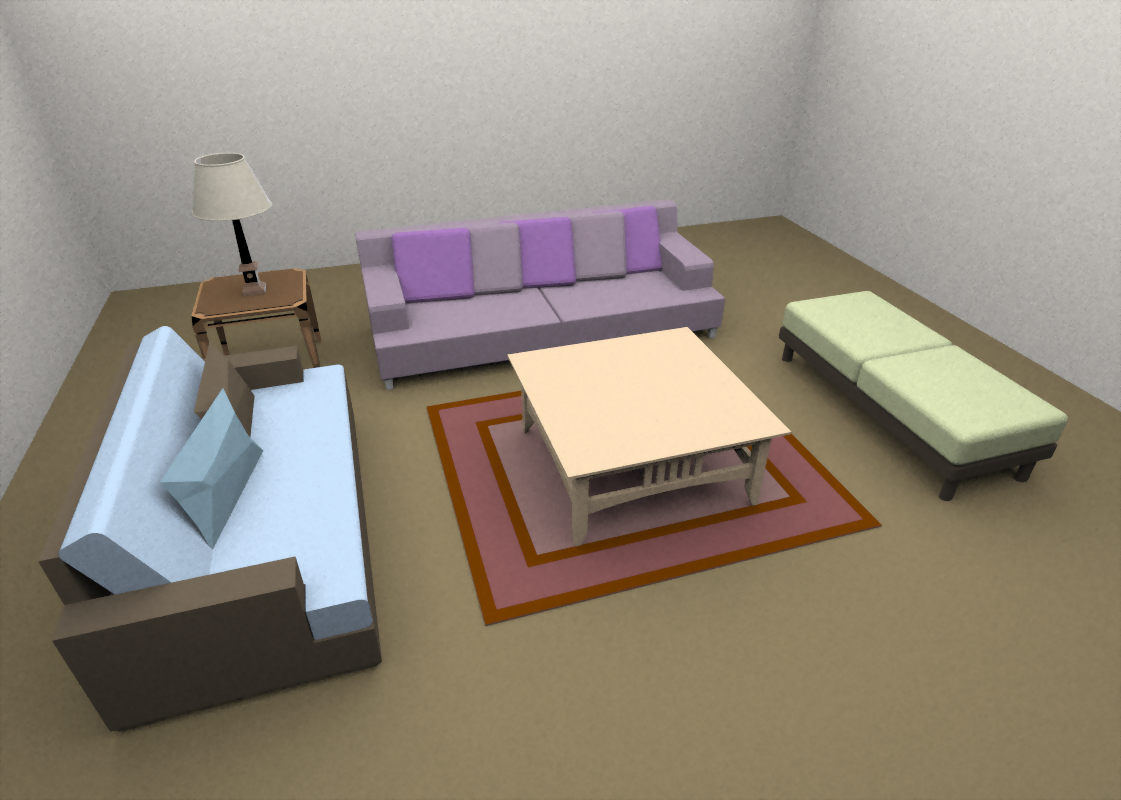
\includegraphics[width=.23\linewidth]{figs/3dscene/original_pbrt}&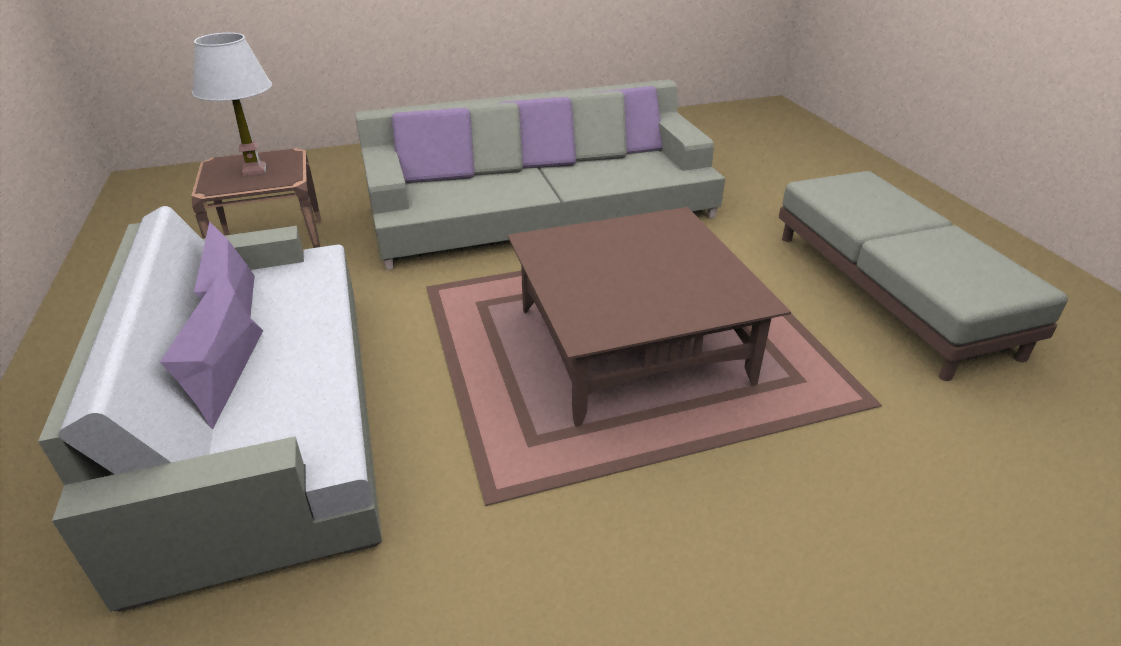
\includegraphics[width=.23\linewidth]{figs/3dscene/recolored_17_pbrt}&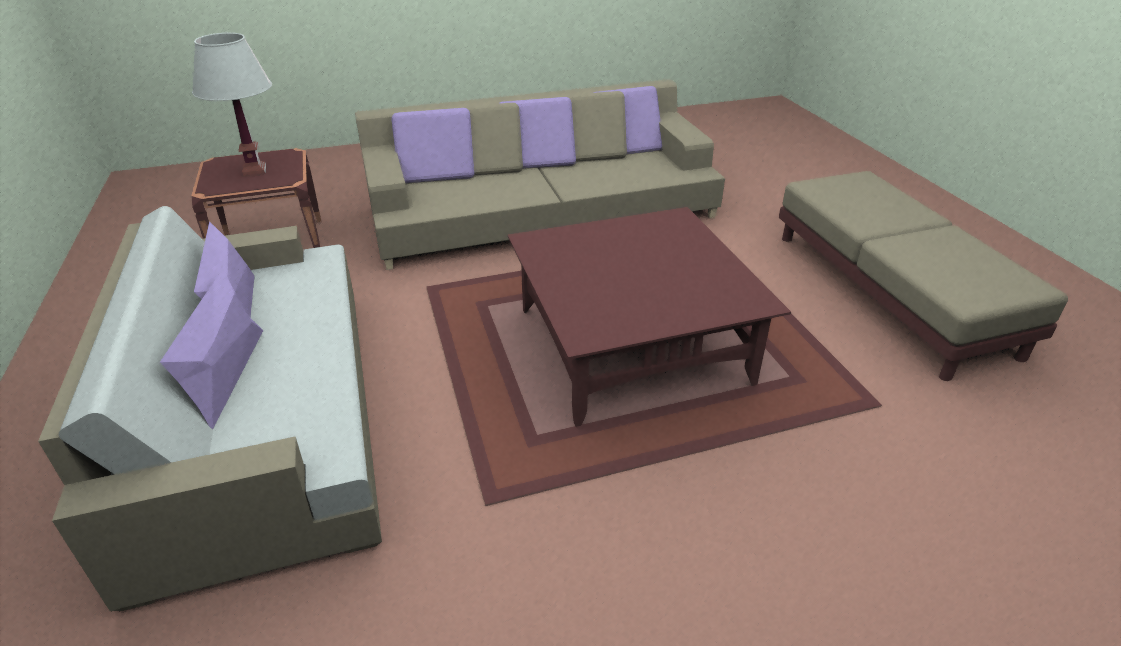
\includegraphics[width=.23\linewidth]{figs/3dscene/recolored_03_pbrt}&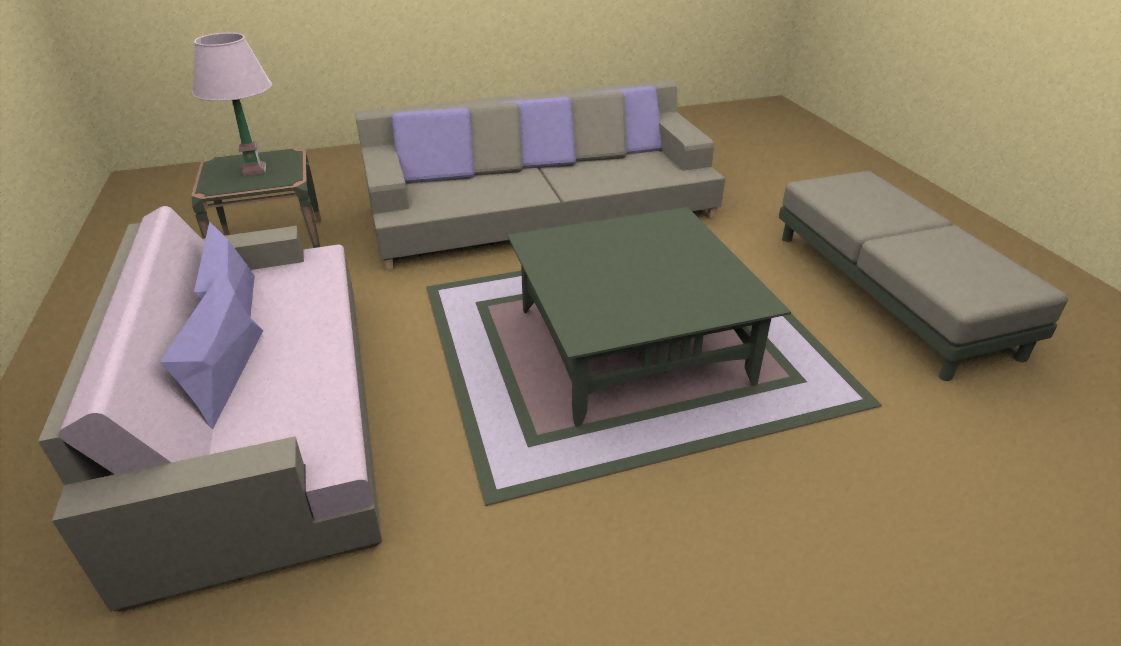
\includegraphics[width=.23\linewidth]{figs/3dscene/recolored_15_pbrt}\vspace{0.4em}\\
\end{tabular}

\caption{A poorly color-coordinated 3D scene is recolored using our model. Using the original coloring as a soft constraint, our model suggests multiple novel recolorings. (Top) Diffuse material coefficients for each object. (Bottom) Final renderings of each scene.}
\label{fig:sceneRecoloring}
\vspace{-1.0em}
\end{figure*}

\paragraph{Fashion design}
Our model can also adapt the colorings of clothing items to fit different people. Figure~\ref{fig:fashion} shows a shirt recolored to match different hair, eye, and skin tones. The hair, skin, eyes, and lips of the 3D person model were manually quantized to a single color; the resulting texture atlas functions as a recolorable pattern template. Fixing the colors of the hair, skin, eyes, and lips constrains the inference process to produce suitable colorings for a person with those physical attributes. It should be possible to apply a similar procedure to photographic images, though those inputs may require an intrinsic image decomposition to separate shading from reflectance~\cite{IntrinsicImages}.

\begin{figure}[ht!]
\centering
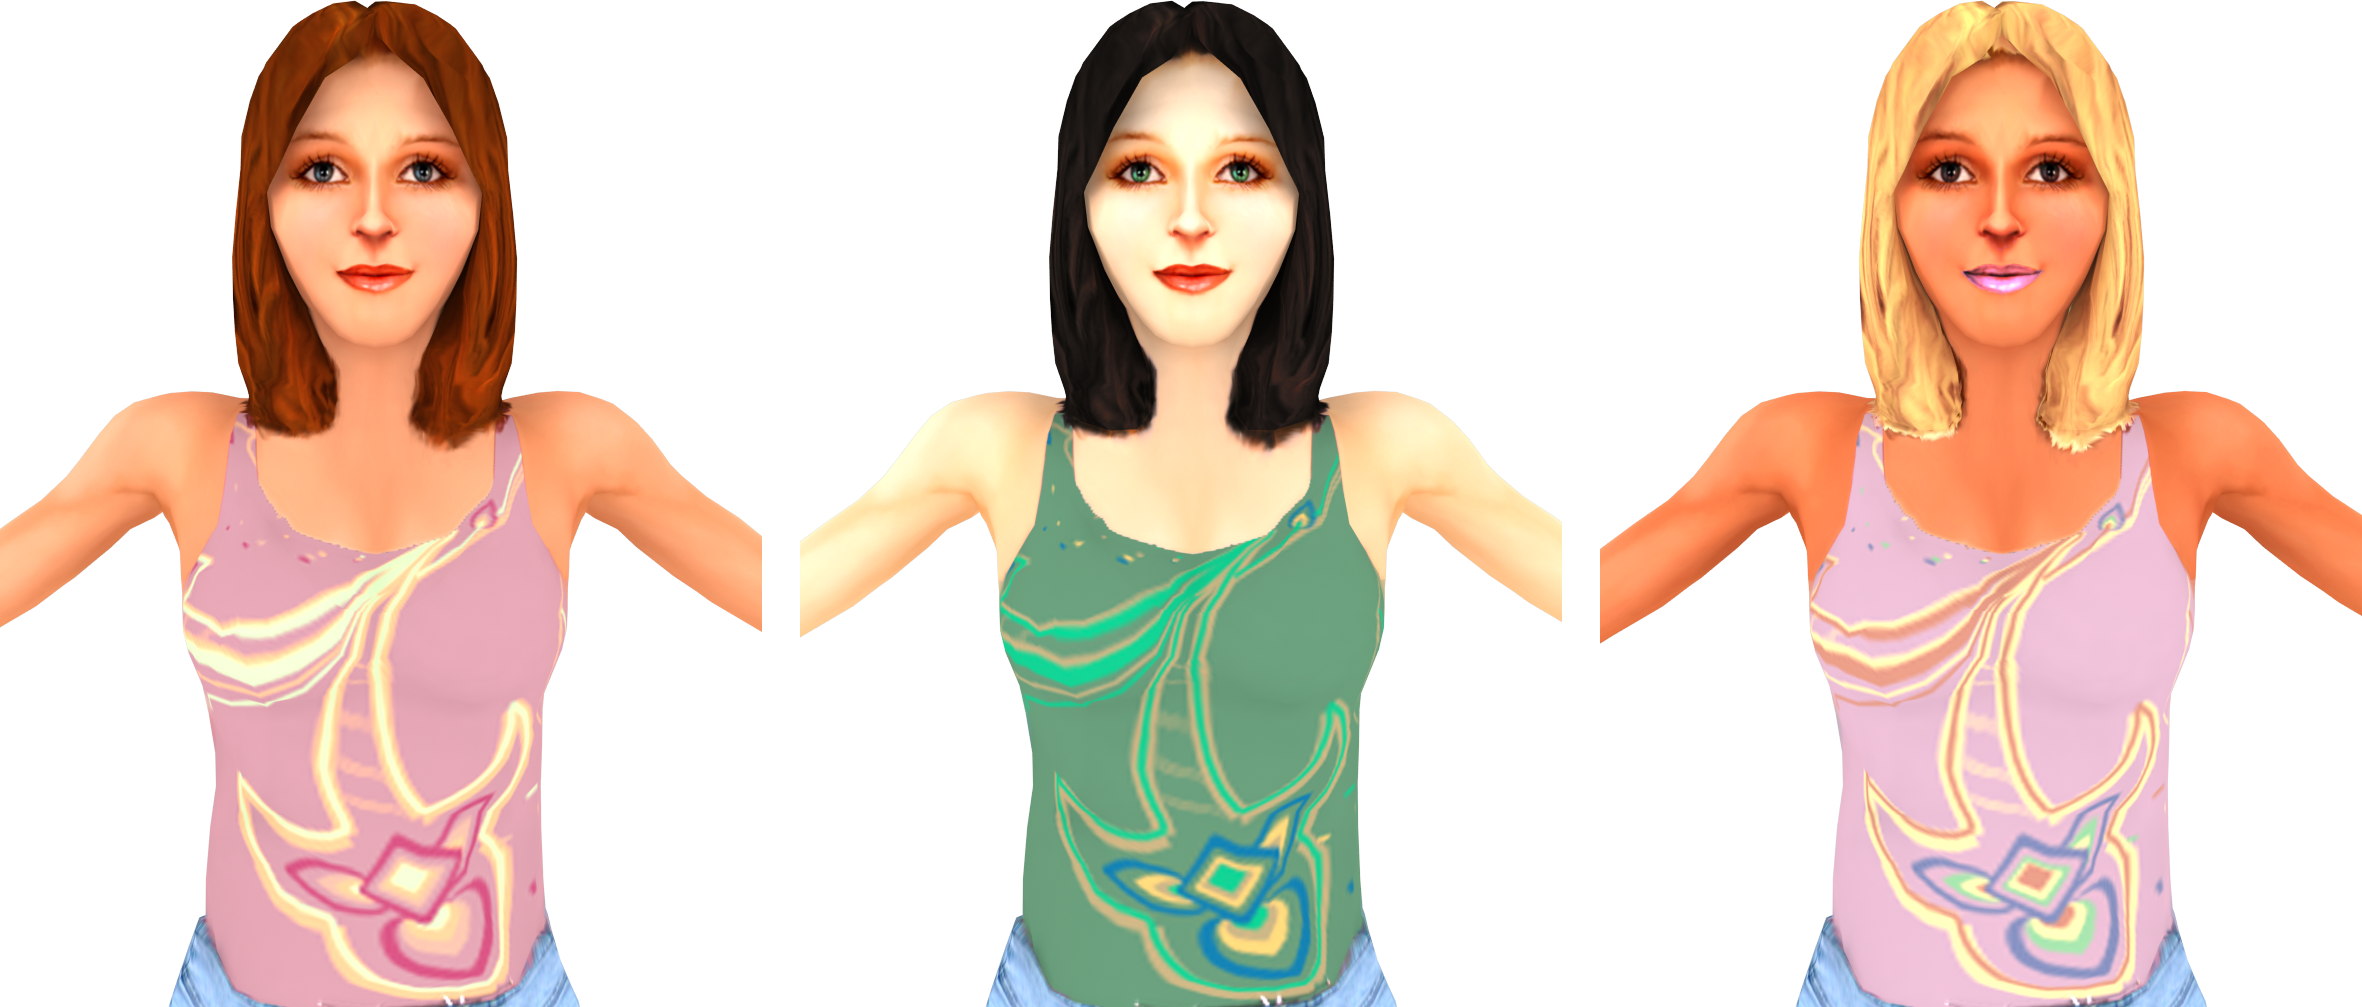
\includegraphics[width=\columnwidth]{figs/fashion/composite}
\caption{Using our model to colorize a patterned shirt for different people. The hair, skin, eye, and lip colors are treated as fixed constraints, which encourage the model to produce compatible colorings via adjacencies and long-range dependencies.}
\label{fig:fashion}
\end{figure}

\subsection{Performance}

The time required to generate coloring suggestions varies depending on the visual complexity of the pattern. Using the parallel tempering parameters described at the beginning of this section, the average sampling time was 73.0s to retrieve 20 MMR-diversified results for a single input pattern on a 2.67GHz Intel Core i7. Sampling is dominated by the probabilistic inference phase, which on average accounts for 83\% of the total running time.

Enabling real-time coloring suggestions would benefit many of the applications demonstrated in this paper, and there are several avenues for improving the performance of our unoptimized, JVM-based prototype to this end. We could leverage the massive parallelism of graphics hardware to speed up parallel tempering, as was done in related work on automatic furniture layout~\cite{MerrellFurnitureLayout}. We could also improve the convergence of the individual MCMC chains via gradient-based proposals, as in Hamiltonian MCMC~\cite{HamiltonianMCMC}. Prior work has shown the feasibility of computing the gradients of programmatically-expressed distributions using automatic differentation~\cite{AutoDiff}. 